% Secondary analyses, robustness and placebo checks. Every number is a macro.
% Runs: sec-cemn, sec-dube, rob-base-2023q4, rob-pre-ab257, rob-pool, rob-7225, rob-final-quarters,
% plc-nonff, plc-722511, anticip, event-path; posthoc part (c) for the employment drift (D7).
% The wage drift (r-ph-wage-*) is cited only in Section 6.4 next to the Georgia check (r-ph-h1-joint).
\section{Secondary analyses, robustness and placebo checks}
\label{sec:robustness}

Every check planned in Section~\ref{sec:robust-plan} was run once and is reported here, whatever it
shows. Table~\ref{tab:robust} collects the employment estimates. None of the checks that can
qualify the headline gives a sign category different from the primary's: all are
``inconclusive''. One check fails: the placebo outcome.

\begin{table}[tbp]
\centering
\caption{Employment estimates of the secondary analyses, robustness and placebo checks (log points)}
\label{tab:robust}
\small
\begin{tabularx}{\linewidth}{@{}>{\raggedright\arraybackslash}Xrrrl@{}}
\toprule
Specification & Estimate & 95\% interval & 90\% interval & H2-rule label \\
\midrule
Primary, \cand{DDT-POPW-E-R50} (H2) & $\HTwoAtt$ & $[\HTwoLoNinetyFive,\ \HTwoHiNinetyFive]$ & $[\HTwoLoNinety,\ \HTwoHiNinety]$ & inconclusive \\
\addlinespace
\multicolumn{5}{@{}l}{\emph{Named secondary analyses}} \\
S1, detrended DD of Clemens and coauthors, R50 aggregate & $\SOneAtt$ & $[\SOneLo,\ \SOneHi]$ & $[\SOneLoNinety,\ \SOneHiNinety]$ & inconclusive \\
S1 without the trend & $\SOneSimpleAtt$ & $[\SOneSimpleLo,\ \SOneSimpleHi]$ & & \\
S2, SDID of Dube, per capita, D20 & $\STwoAtt$ & $[\STwoLo,\ \STwoHi]$ & $[\STwoLoNinety,\ \STwoHiNinety]$ & inconclusive \\
\addlinespace
\multicolumn{5}{@{}l}{\emph{Robustness checks (selected estimator)}} \\
Base 2023Q4 (Dube's), 2024Q1 dropped & $\RobBaseFourAtt$ & $[\RobBaseFourLo,\ \RobBaseFourHi]$ & $[\RobBaseFourLoNinety,\ \RobBaseFourHiNinety]$ & inconclusive \\
Base 2022Q2, before AB 257 & $\RobPreABAtt$ & $[\RobPreABLo,\ \RobPreABHi]$ & $[\RobPreABLoNinety,\ \RobPreABHiNinety]$ & inconclusive \\
Other pool (D20) & $\RobPoolAtt$ & $[\RobPoolLo,\ \RobPoolHi]$ & $[\RobPoolLoNinety,\ \RobPoolHiNinety]$ & inconclusive \\
All restaurants (NAICS 7225), four suppressed donors dropped & $\RobAllRestaurantsAtt$ & $[\RobAllRestaurantsLo,\ \RobAllRestaurantsHi]$ & $[\RobAllRestaurantsLoNinety,\ \RobAllRestaurantsHiNinety]$ & inconclusive \\
\quad all donors, 2024Q4 dropped & $\RobAllRestaurantsAllDonorsAtt$ & $[\RobAllRestaurantsAllDonorsLo,\ \RobAllRestaurantsAllDonorsHi]$ & & \\
Final data only, 2024Q2--2025Q4 & $\RobFinalAtt$ & $[\RobFinalLo,\ \RobFinalHi]$ & $[\RobFinalLoNinety,\ \RobFinalHiNinety]$ & inconclusive \\
\addlinespace
\multicolumn{5}{@{}l}{\emph{Placebo outcomes (selected estimator)}} \\
Employment outside 722513 & $\PlcNonffAtt$ & $[\PlcNonffLo,\ \PlcNonffHi]$ & & fails \\
Full-service restaurants (722511), not a clean placebo & $\PlcFullServiceAtt$ & $[\PlcFullServiceLo,\ \PlcFullServiceHi]$ & & report only \\
\bottomrule
\end{tabularx}

\medskip
\begin{minipage}{\linewidth}\footnotesize
\emph{Notes:} Pooled 2024Q2--2026Q1 effects on seasonally adjusted log employment of California's
private NAICS 722513 (other rows as stated), base 2023Q3 unless stated. Each label is the one the
H2 rule gives, and none is the headline. S1 and S2 use their own critical values (S2 with the D20
SDID floor), the other-pool check its own, and the remaining rows the selected candidate's
employment critical values with $t$ at each run's own $\nu$. Blank cells: not reported by the run.
\end{minipage}
\end{table}

\subsection{The two published approaches}
\label{sec:rob-secondary}

\paragraph{S1, the detrended comparison of Clemens and coauthors.} Re-estimated with our 2023Q3
base, pooled post window and inference, S1 gives $\SOneAtt$ log points ($\SOnePct$ percent), with
a 95 percent interval from $\SOneLo$ to $\SOneHi$: ``inconclusive''. Their placebo rank $p$-value
is $\SOneRankP$ (one-sided). Without the trend the estimate is $\SOneSimpleAtt$ (rank
$p = \SOneSimpleRankP$). The cross-check against print reproduces their September-to-September
fixed-horizon estimates for 2023--2025 with their 48-state pool at $\CemnFhSimple$ index points
(simple) and $\CemnFhDetr$ (detrended), against $-2.74$ and $-3.72$ in
\citet[Table~3, Panel~B]{clemens2026employment}: both of ours are more negative than the printed
values, by $\CemnFhSimpleDiff$ and $\CemnFhDetrDiff$ points, a difference we have not traced.

\paragraph{S2, the SDID of Dube.} With our timing S2 gives $\STwoAtt$ log points ($\STwoPct$
percent), with a 95 percent interval from $\STwoLo$ to $\STwoHi$: ``inconclusive''. Its interval
is the narrowest of the three in Table~\ref{tab:headline}, but S2 also behaves worst for California
before the law: its six pseudo-ATTs are all positive, from $\CaSTwoSeventeenQTwoTau$ to
$\CaSTwoSixteenQTwoTau$ log points, the root mean square of California's six $t$ statistics is
$k = \KDiagSTwo$, and California's upper one-sided test rejects at a share $\RejSTwoMaxCAUp$ of
the pseudo-dates even with the maximum standard error and the SDID floor. The narrower interval is
therefore not support for a near-zero effect. S2's wage effect with the employment weights reused,
as Dube does, is $\STwoWage$ (95 percent interval $\STwoWageLo$ to $\STwoWageHi$); for the same
reason it is not an independent confirmation of the first stage. Under Dube's own timing our SDID
gives $\DubeTimingEmp$ ($100\times$ log points; scaled placebo standard error $\DubeTimingSe$),
against $-0.26$ (0.54) in \citet[Table~1, Panel~A]{dube2026labor}, a difference of
$\DubeTimingEmpDiff$, and a wage effect of $\DubeTimingWage$ against 6.99 (difference
$\DubeTimingWageDiff$). Our SDID includes an intercept and separate penalties and uses our own
seasonal factors, so this cross-check measures the combined difference from his implementation.

\subsection{Robustness checks}
\label{sec:rob-checks}

Moving the base to Dube's 2023Q4 gives $\RobBaseFourAtt$; moving it before AB 257, to 2022Q2, gives
$\RobPreABAtt$ with a wider interval; the trend is then extrapolated over a longer horizon. The other pool,
D20, gives $\RobPoolAtt$. Dropping the preliminary 2026Q1 gives $\RobFinalAtt$, so the one new
quarter moves the pooled estimate little. All four are ``inconclusive'', with point estimates
between $\RobPreABAtt$ and $\RobBaseFourAtt$, around the primary's $\HTwoAtt$.

For all restaurants (NAICS 7225) the estimate is $\RobAllRestaurantsAtt$ with the four donors
whose 2024Q4 row is suppressed dropped, and $\RobAllRestaurantsAllDonorsAtt$ with all donors and
2024Q4 dropped from the post window; both intervals contain zero. A 722513 decline with no 7225
decline was to point to reclassification or substitution toward other restaurants; neither the
722513 nor the 7225 estimate is distinguishable from zero, so the check cannot speak to it.

\subsection{Placebo outcomes}
\label{sec:rob-placebo}

Employment in all covered industries except 722513 ran above its counterfactual by
$\PlcNonffAtt$ log points ($\PlcNonffPct$ percent), with a 95 percent interval from $\PlcNonffLo$
to $\PlcNonffHi$ that excludes zero. By the pre-specified rule the H2 label is qualified as not
separable from a California-wide shock. The deviation is about as large as the H2 estimate and of
the opposite sign: if the same California-wide deviation reached 722513, the H2 estimate is biased
toward zero or upward, not toward a decline. No numerical adjustment was pre-specified and none is
made. The comparison therefore does not hold for California's aggregate labour market, which is
falsification check (iii) of the identifying assumption (Section~\ref{sec:assumption}). With two
placebo outcomes, one failure by chance alone had a probability of about 0.10; we do not discount
the failure for that.

Full-service employment (722511), reported only because covered chains are also coded there, gives
$\PlcFullServiceAtt$, with an interval from $\PlcFullServiceLo$ to $\PlcFullServiceHi$. As stated in
the plan, a null estimate here does not validate the design.

\subsection{Anticipation}
\label{sec:rob-anticip}

Between signing and the effective date (2023Q4--2024Q1), against the 2023Q3 base, the employment
effect is $\AnticipEmp$ (95 percent interval $\AnticipEmpLo$ to $\AnticipEmpHi$) and the wage
effect $\AnticipWage$ ($\AnticipWageLo$ to $\AnticipWageHi$); neither is tested. The wage interval
uses H1's decision-set critical value $c_{\mathrm{hi}}(0.975)$, so it is wide on the negative side
(Section~\ref{sec:res-inference}).

\subsection{The event path}
\label{sec:rob-event}

Figure~\ref{fig:event} shows the quarterly gap between California and the selected counterfactual.
For the trend-adjusted estimator the 2022Q1--2023Q3 gaps are residuals around the fitted trend,
so they test only curvature: their root mean square is $\EventEmpRmsGap$ for employment and
$\EventWageRmsGap$ for wages, and $\EventEmpBandsExcl$ of the seven employment and
$\EventWageBandsExcl$ of the seven wage bands exclude zero. This is not a pre-trend test. The
out-of-fit evidence before the law is the 2014--2019 segment. For employment, the gap there rises
from $\PhDriftEmpGapStart$ in 2014Q1 to $\PhDriftEmpGapEnd$ in 2019Q4, a slope of
$\PhDriftEmpSlope$ per quarter and a root mean square of $\PhDriftEmpRms$ (post hoc, deviation
D7). If that relative trend applied after 2023Q3, it would amount to about
$\PhDriftEmpImpliedPost$ log points at the post window's mean horizon, so the H2 estimate would be
biased toward zero or upward by about that amount and the counterfactual would imply a larger
decline; this is the same direction as the placebo outcome. The extrapolation is not a test, the
2014--2019 segment contains California's own general minimum-wage ramp, and the H2 label does not
change. The wage panel's out-of-fit segment bears on H1 and is reported in
Section~\ref{sec:res-posthoc}, next to the check of H1's critical value. The bands of the figure
are pointwise and use the H2 critical values in both panels, and no label is read from it; in
particular a wage band that excludes zero is not evidence against the H1 verdict.

\begin{figure}[tbp]
\centering
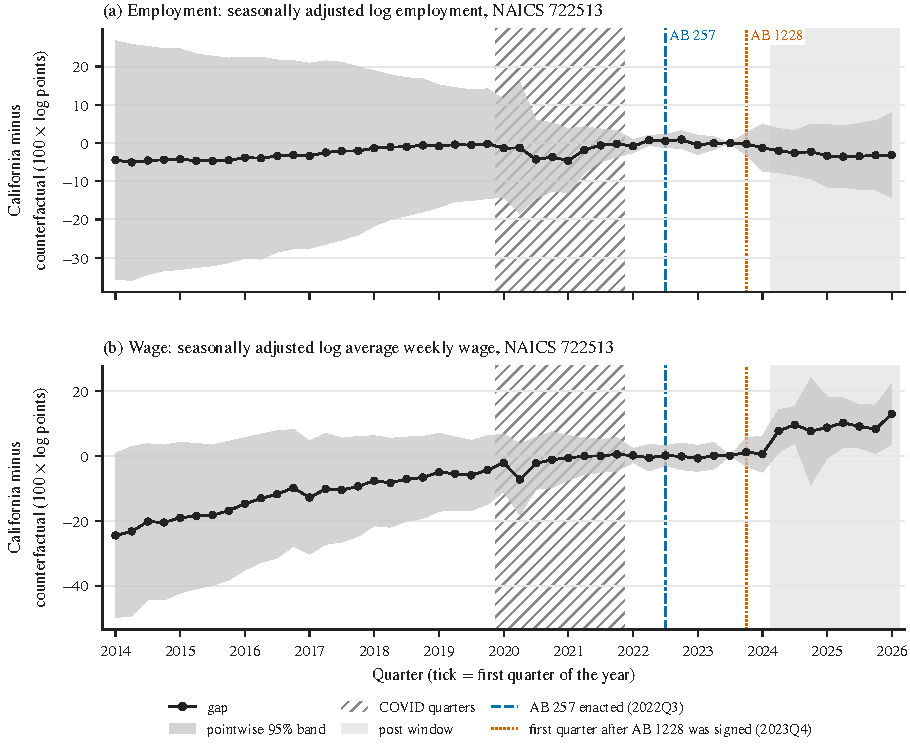
\includegraphics[width=0.85\linewidth]{figures/fig_event.pdf}
\caption{Quarterly gap between California and its estimated counterfactual, 2014Q1--2026Q1, for the
primary candidate \cand{DDT-POPW-E-R50}. Panel (a): seasonally adjusted log employment, NAICS
722513; panel (b): seasonally adjusted log average weekly wage, same estimator, weighting and pool,
with the trend fitted on the wage. Each point is California's outcome minus the counterfactual,
fitted with the base quarter 2023Q3, in $100\times$ log points. Shaded band: pointwise 95 percent
interval with $\mathrm{SE} = \max(\SEs, \SEn)$ from the donors' placebo gaps at that quarter and
the H2 critical values ($t$ at $\nu = \HTwoNu$, $c_{\mathrm{hi}}(0.975) = \CritHTwoHiNinetySevenFive$)
in both panels. H1 is decided by run \cand{h1-wage}, whose one-sided critical value
$\HOneCrit$ is far above $\CritHTwoHiNinetySevenFive$, so on the upper side the wage bands are
narrower than the H1 test. Hatched: COVID quarters, excluded from every fit. Light shading: the
post window. Dashed line: 2022Q3 (AB 257 enacted); dotted line: 2023Q4 (first quarter after AB
1228 was signed). For DDT the 2022Q1--2023Q3 gaps are residuals around the fitted trend (curvature
only); the 2014--2019 segment is outside the trend's fit. The bands are pointwise, no part of the
figure is a pre-trend test, and no hypothesis label is read from it. Run \cand{fig-event}.}
\label{fig:event}
\end{figure}
